\chapter{Conception du système}

\section{Introduction}
%Of course talk here about what the chapter is about
Durant ce chapitre, nous allons présenter en détail les étapes de conceptions de notre système, tout d'abord une architecture générale est présentée et décortiquée, ensuite chaque module du système sera détaillé du point de vue des composants qui le constitueraient en donnant un maximum de détails tout en restant assez concis. Une conclusion viendra clôturer ce chapitre pour introduire ensuite le suivant.
\section{Architecture du système}
%Try to be as precise as possible while letting room for more details to the next sections
\begin{figure}[H]
	\label{spa_arch}
	\centering
	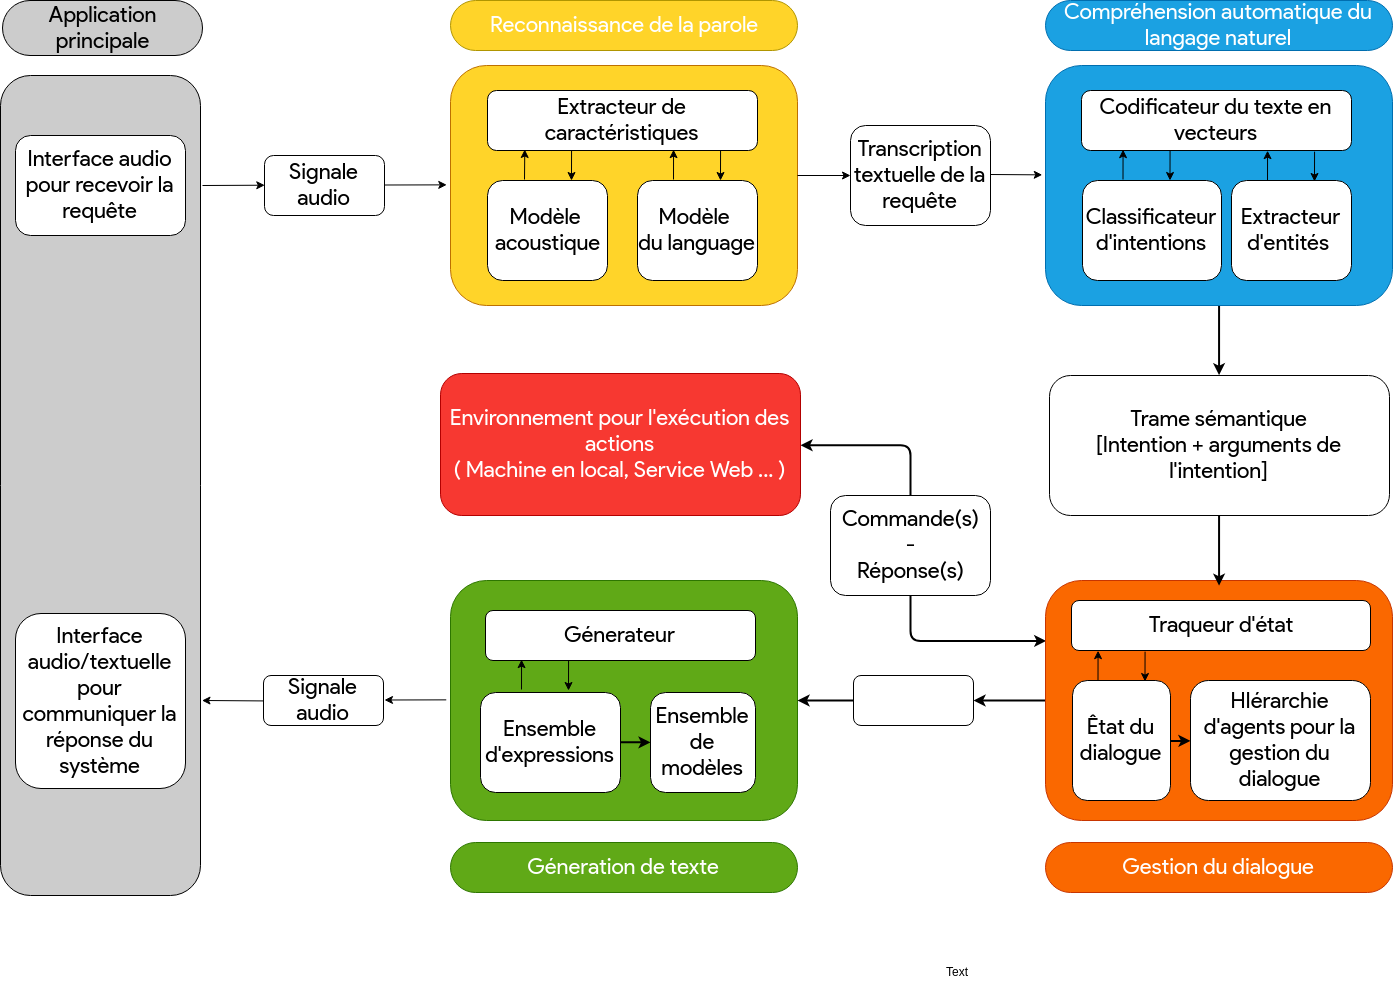
\includegraphics[width=0.88\linewidth]{images/SPA_architecture.png}
	\caption{Architecture générale de notre système}
\end{figure}
\paragraph{}
Comme montré dans la figure ci dessus (\ref{spa_arch}) et comme cité dans le chapitre précédent (voir \ref{spa_schem_section}) le système se présente comme l'interconnexion de cinq parties dont une interface \footnote{ici nous par interface nous entendons le sens abstrait du terme et non obligatoirement  dans le sens interface graphique} et quatre modules internes, chaque module forme ainsi un maillon d'une chaîne qui représente une partie du cycle de vie du système. L'architecture du système est une pipeline (chaîne de traitement) de processus qui s'exécutent de manière indépendante mais qui font circuler un flux de données entre eux dans un format préalablement décidé (voir \ref{spa_diagram}). Nous pouvons séparer ces parties en deux catégories :
	\subsection{Couche utilisateur}
%	What the users sees as input/output and the interfaces that are available for him
	Cette couche représente ce que l'utilisateur peut voir comme entrée/sortie et les interfaces qui lui sont accessibles, puisque l'assistant est un processus qui communique majoritairement avec l'utilisateur à travers des échanges verbaux, nous avons pensé à implémenter l'interface du système comme une processus qui s'exécute en arrière plan et qui attend d'être activer (pour le moment par un événement physique, c.à.d clique sur un bouton/icône ou raccourci clavier), l'assistant pourra ensuite répondre en affichant un texte à l'écran qui sera vocalement synthétisé envoyer à l'utilisateur via l'interface de sortie de son choix (afficher le texte et sa transcription vocale pourrait palier au manque d'un périphérique de sortie audio).
	\subsection{Couche système }
%	What the users doesn't see and what are the main components of the system
	Cette couche quant à elle représente ce que l'utilisateur ne voit pas et fait donc partie du fonctionnement interne du système, elle regroupe les quatre grandes étapes d'un cycle de vie pour une commande reçu de la couche utilisateur. Comme mentionné dans le chapitre précédent (voir \ref{spa_life_cycle}), la requête passe par un module de reconnaissance de la parole, qui traduira en texte le signale audio correspondant à la requête, le module suivant va extraire l'intention de l'utilisateur et ses arguments (par exemple \textit{"open the home folder"} pourrait donner  une intention dy type  \textit{open\_file\_desire[file\_name="home",parent\_directory="?"]}), le gestionnaire de dialogue gardera trace de l'ensemble des échanges effectués entre l'utilisateur et l'assistant et essayera d'atteindre le but final formuler par la requête (la plus récente ou la plus ancienne), pour ce faire il aura besoin d'interagir avec ce qu'on a appelé un environnement d'exécution, qui peut être la machine où l'assistant réside ou une API \footnote{Application programming interface ou interface de programmation applicative } qui aura accès à un service a distance (sur internet par exemple) ou locale (dans un réseau domestique). Finalement une action spéciale qui servira à informer l'utilisateur sera envoyé au module suivant pour être transformé en son équivalant en langage naturel, puis le texte sera vocalement synthétiser et envoyé vers l'interface de sortie de l'application.

\section{Module de reconnaissance automatique de la parole}
	\subsection{Architecture du module}
	\subsection{Modèle acoustique}
		\subsubsection*{Données d'apprentissage}
%		audio files and their transcriptions
		Fichiers audios avec leurs transcriptions en texte
		\subsubsection*{Type du modèle}
%		Deep neural network trained with end to end paradigm
		Réseau de neurones profond avec apprentissage de bout en bout
	\subsection{Modèle de la langue}
		\subsubsection*{Données d'apprentissage}
%		Talk about the process of data gathering (github readmes and cleaning process)
		Parler de la procédure de récolte des données (provenances, qualité, quantité ...)
		\subsubsection*{Type du modèle}
		N-grams

\section{Module de compréhension automatique du langage naturel }
	\subsection{Architecture du module}
	\subsection{L'analyse sémantique}
	\subsection{Analyse sémantique basée sur les grammaires de dépendances}
	\subsection{Analyse sémantique avec apprentissage automatique}
		\subsubsection{Les données d'apprentissage}
		Construction et enrichissement du corpus 
		\subsubsection{Modèle utilisé}
	
	
\section{Module de gestion du dialogue}
	\subsection{Architecture du module}
	\subsection{Les ontologies du système}
		Here talk about the graph encoder 
		\subsubsection*{Explorateur de fichiers}
	\subsection{Les simulateurs d'utilisateurs}
		\subsubsection*{Explorateur de fichiers}
	\subsection{Modèles d'apprentissage}
		\subsubsection*{L'agent coordinateur}
		\subsubsection*{Les sous agents}

\section{Module de génération du langage naturel}
	Reste à décider
\section{Conclusion}	